\chapter{Time series analysis and forecasting}

In this chapter we will explore time series analysis and forecasting techniques. We will start with linear models and move on to more complex ones.

In \textbf{time series\index{time series}} data we don't really have a population, instead we have a data generating process, that we are sampling at certain points in time. Population would mean all observations at any given time, which would mean an infinite number of observations.


\begin{figure}[htbp]
    \begin{center}
        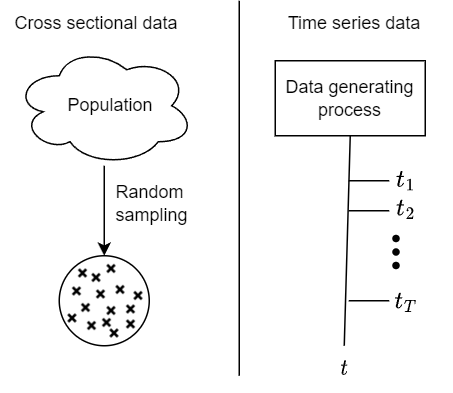
\includegraphics[width=250pt]{../img/09-time-series.png}
        \caption{Figure 9.1:  Cross sectional data (left) vs time series data (right)}
    \end{center}
\end{figure}


\section{Linear models for time series analysis}

In the case of linear regression, the Gauss-Markov conditions are required for OLS to provide the best linear unbiased estimator (BLUE). However, for time series analysis, other linear models may be more appropriate.

\subsection{Assumption of linear models for time series}

Time series linear models require some modifications to the Gauss-Markov assumptions, such as the inclusion of strict exogeneity instead of weak exogeneity. Nevertheless, in practice, when the sample size is large enough, similar conditions apply.

In cross-sectional data analysis, the assumption is that the samples are independent and identically distributed (i.i.d). However, in time series analysis, the assumption of independence no longer holds due to temporal dependence between the observations. Instead of assuming i.i.d, we introduce the concept of \textbf{weak dependence\index{weak dependence}}.

A time series is considered weakly dependent if the correlation between a value and a lagged value tends to zero as the lag tends to infinity:
\[Corr(x_t, x_{t+h}) \rightarrow 0, h \rightarrow \infty\]

This condition serves as a replacement for the random sampling assumption in cross-sectional data. Since the correlation becomes minimal as the lag increases, we can treat the observations as if they were i.i.d, allowing us to perform inference.

Some of the linear models we can use for time series require that the time series is \textbf{stationary\index{stationary}}. The conditions for stationary time series are

\begin{enumerate}
    \item \textbf{Stationary in mean\index{Stationary in mean}}: the expectation of all the variables is a finite constant, and not a function of time. \[E[x_t] = \mu < \infty, E[x_t] \neq f(t)\] This means there is no gradual growth with time in our variables.
    \item \textbf{Stationary in variance\index{Stationary in variance}}: the variance of all the variables is a finite constant, and not a function of time\textit{ }\[Var(x_t) = \sigma^2 < \infty, Var(x_t) \neq f(t)\]
    \item \textbf{Covariance stationary\index{Covariance stationary}}: The covariance of a value of the time series and one which is lagged needs to be a function of the lag and not time. \[Cov(x_t, x_{t+h}) = f(h) \neq f(t)\]
\end{enumerate}

These conditions ensure that the statistical properties of the time series remain constant over time


\begin{figure}[htbp]
    \begin{center}
        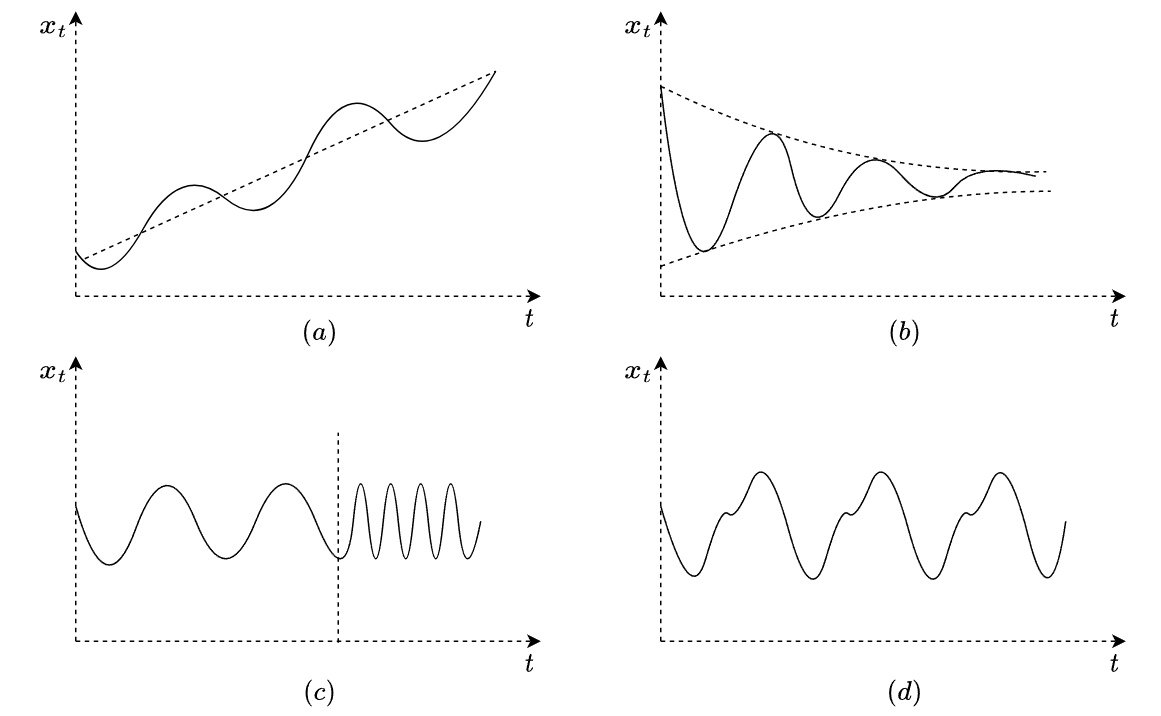
\includegraphics[width=250pt]{../img/09-stationary.png}
        \caption{Figure 9.2:  (a) Non-stationary in mean, (b) non-stationary in variance, (c) time-varying autocovariance (non covariance stationary), (d) stationary time series}
    \end{center}
\end{figure}


If we try to apply linear model to a non stationary variable or a predictor variable is non stationary, the following issues might arise:
\begin{itemize}
    \item When we try to model a variable \(y\) on \(x\), if only \(y\) is non stationary, there is no linear relationship we could describe (\(y\) has a slope but \(x\) does not, so there is no \(y = \beta_0 + \beta_1 x\) that can model the relationship)
    \item If both \(x\) and \(y\) are not stationary, but the degree of growth is different, e.g. \(x\) has a linear growth but \(y\) has an exponential growth, we arrive to the same problem where we are not able to model one variable with another using linear model.
    \item Even if both \(x\) and \(y\) have a linear slope, the relationship between the independent and dependent variable might simply be sporadic correlation (accidental). We could model a growing variable with another, even if there is no relationship. A famous example is a study in 1970 about the increase in margarine consumption and divorce rate in the US.
\end{itemize}

There is also a theoretical reason, which is related to the law of large numbers and the central limit theorem, that we will not explore here.

\subsection{The MA model}

We call a data generating process \textbf{moving average\index{moving average}} if the model has the following form:

\[\operatorname{MA}(k): x_t = \epsilon_t + \theta_1\epsilon_{t-1}  + ... + \theta_k\epsilon_{t-k} \]

where \(\theta_1, ..., \theta_k\) are the weights of the model, and \(\epsilon_{t-1},...,\epsilon_{t-k}\) are i.i.d error terms:

\[\epsilon_{t-1},...,\epsilon_{t-k} \sim i.i.d(0, \sigma^2)\]

The moving average process is stationary and weekly dependent. We can simply find this by applying the model equation to the conditions. Applying to MA(1):

\begin{enumerate}
    \item \(E[x_t] = E[\epsilon_t] + \theta E[\epsilon_{t-1}] = 0\) — constant mean, not a function of time
    \item \(Var(x_t) = Var(\epsilon_t) + \theta^2 Var(\epsilon_{t-1}) = \sigma^2(1 + \theta^2)\) — constant variance, not a function of time
    \item \(\operatorname{Cov}(x_t, x_{t-1}) = \operatorname{Cov}(\epsilon_t + \theta\epsilon_{t-1}, \epsilon_{t-1} + \theta\epsilon_{t-2})\)

We can expand the covariance same as multiplication, but we know error terms are independent, so we only need to consider the recurring error term \(\epsilon_{t-1}\):

\(= \theta \operatorname{Cov}(\epsilon_{t-1}, \epsilon_{t-1}) = \theta Var(\epsilon_{t-1}) = \theta \sigma ^2\)

For a lag \(h\) larger than \(1\)

\(\operatorname{Cov}(x_t, x_{t-h}) = 0\)

Overall it's a function of the lag and not of time
\end{enumerate}

Similarly the correlation will also become \(0\) for lag larger than the lag in the model, making it weakly dependent.

\subsection{The AR model}

The \textbf{auto regressive\index{auto regressive}} or AR model assumes a relationship in the time series between a point in time and a given lag.

\[\operatorname{AR}(k): x_t = \rho_0 + \rho_1 x_{t-1} + ... + \rho_k x_{t-k} + \epsilon\]

Where \(\rho_1, ..., \rho_k\) are the model parameters, \(\epsilon\) is the error term, which is i.i.d with a mean of \(0\) and a variance of \(\sigma^2\):

\[\epsilon \sim i.i.d(0, \sigma^2)\]

The AR model is stationary under certain conditions. If we examine AR(1) and apply it for the conditions of stationary.

\begin{enumerate}
    \item \textbf{Stationary in mean\index{Stationary in mean}}:

\(E[x_t] = \rho_0 + \rho_1 E[x_{t-1}] + E[\epsilon_t]\) \\
\(E[\epsilon_t]\) is simply 0 from the definition. In order for the process to be stationary it must hold that \(E(x_t) = E(x_{t-1})\)  (we will reuse this several times below), substituting these: \\
\(E[x_t] = \rho_0 + \rho_1 E[x_t] \Leftrightarrow\) \\
\[E[x_t] = {\rho_0 \over 1 - \rho_1}\]

For the process to be stationary, we need \(E[x_t]\) to be finite, which means \[\rho_1 \neq 1\] needs to hold, otherwise it's division by 0.

    \item \textbf{Stationary in variance\index{Stationary in variance}}:

\(Var(x_t)=Var(\rho_0+\rho_1x_{t-1}+\epsilon_t)=\rho_1^2V(x_{t-1})+\underbrace{2Cov(x_{t-1},\epsilon_t)}_{=0}+\underbrace{Var(\epsilon_t)}_{\sigma^2}\). In order for the process to be stationary it must hold that \(Var(x_t) = Var(x_{t-1})\): \\
\(Var(x_t)=\rho^2Var(x_t)+\sigma^2 \Leftrightarrow\)

\[Var(x_t)={\sigma^2 \over 1-\rho_1^2}\]

The variance to be positive and finite, we need \\
\(\rho_1^2<1 \Leftrightarrow\)

\[\vert \rho \vert <1\]

    \item \textbf{Covariance stationary\index{Covariance stationary}}:

We can take result of 1., rearrange the elements:

\(E[x_t] = {\rho_0 \over 1 - \rho_1}\) \\
\(\rho_0 = (1 - \rho_1)E[x_t]\) \\
And use this to change the center of the process (original AR(1) formula), removing \(\rho_0\):\\
\(x_t-E(x_t)=\rho_1(x_{t-1}-E(x_t))+\epsilon_t\)

Since it's a recursive function and because \(E(x_t) = E(x_{t-1})\), we can substitute \(x_{t-1}-E(x_t)\) with \(\rho_1(x_{t-2}-E(x_t))+\epsilon_t\):

\(x_t-E(x_t)=\rho_1^2(x_{t-2}-E(x_t))+\rho_1\epsilon_{t-1} + \epsilon_t\)

Repeating \(h\) times:

\(x_t-E(x_t)=\rho_1^k(x_{t-h}-E(x_t))+\sum_{i=0}^{h-1}\rho_1^i\epsilon_{t-i}\)

Shifting by \(h\)  (note that again we don't need to update \(E(x_t)\))

\(x_{t+h}-E(x_t)=\rho_1^k(x_{t}-E(x_t))+\sum_{i=0}^{h-1}\rho_1^i\epsilon_{t+h-i}\)

Calculating covariance with the shifted value (auto covariance), because there is no relationship between \(x\) and the error terms, \(\sum_{i=0}^{h-1}\rho_1^i\epsilon_{t+h-i}\) becomes \(0\):

\begin{flalign*}
& Cov(x_t-E(x_t), x_{t+h}-E(x_t)) \\
& = Cov(x_t-E(x_t), \rho_1^k(x_{t}-E(x_t))) \\
& = \rho_1^k Cov(x_t-E(x_t), x_t-E(x_t)) \\
& = \rho_1^k Var(x_t-E(x_t)) \\
& \text{Redoing tha calculation for stationary in variance (2) but with centered process, gives the same result:} \\
& = \rho_1^k {\sigma^2 \over 1-\rho_1^2} \text{This has the same condition as the stationary in variance:} \vert \rho \vert <1 \\ && \end{flalign*}
\end{enumerate}

\subsection{AR or MA process}

A process that is stationary in mean and variance can be either an AR or an MA process. To diagnose wheater a process is AR or MA, we can look at the autocorrelation, which is:

\(Corr(x_t, x_{t+h}) = {Cov(x_t, x_{t+h}) \over \sqrt{Var(x_t)Var(x_{t+h})}}\)

Because the process is stationary, the variance is constant, so \(Var(x_t) = Var(x_{t+h})\)

\begin{equation}Corr(x_t, x_{t+h}) = {Cov(x_t, x_{t+h}) \over {Var(x_t)}} \tag{9.1}\end{equation}

For an MA(1) process, for \(h = 1\): \({Cov(x_t, x_{t+h}) \over {Var(x_t)}} = {\theta \sigma ^2 \over \sigma ^2(1 + \theta^2)} = {\theta \over 1 + \theta^2}\). For values larger than 1, it was simply 0:

\begin{equation}Corr_{MA}(x_t, x_{t+h}) = \begin{cases}
{\theta \over 1 + \theta^2} & ,\ h = 1 \\
0 & ,\ h > 1
\end{cases}  \tag{9.2}\end{equation}

For an AR(1) process we found that \(Cov(x_t, x_{t+h}) = \rho^k Var(x_t)\), applying to (9.1) we get:

\begin{equation}Corr_{AR}(x_t, x_{t+h}) = \rho^k  \tag{9.3}\end{equation}

While these results look complex they can be very intuitive in identifying if a process is AR or MA. We can plot a graph of our time series, where on the \(X\) axis we have integers \(1, 2, ...\) representing lag, and for each we plot the auto correlation with that lag. This plot is called a \textbf{correlogram\index{correlogram}}.


\begin{figure}[htbp]
    \begin{center}
        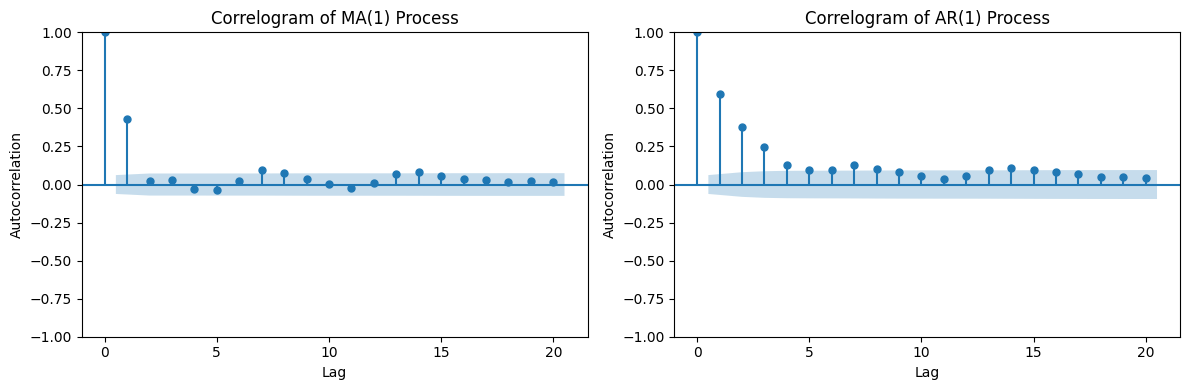
\includegraphics[width=250pt]{../img/09-ma-ar.png}
        \caption{Figure 9.3:  Correlogram of an MA(1) and an AR(1) process.}
    \end{center}
\end{figure}


On \textbf{Figure 9.3\index{Figure 9.3}} we can see the correlogram of an MA(1) and an AR(1) process. All processes have an autocorrelation of 1 with itself with lag 0, so that value does not convey information. The result in (9.2) shows that an MA(1) process will have some value for it's auto correlation at lag \(1\) and \(0\) for lag \(>1\), which is similar to the left side of \textbf{Figure 9.3\index{Figure 9.3}}. The shaded area around the X axis shows statstically insignificant range, correlation values which fall within this range are sampling noise.

An AR(1) model has a non \(0\) auto correlation at lag \(k\), but it:s decaying exponentially as conveyed by (9.3). This same behavior is visible on the right hand side of \textbf{Figure 9.3\index{Figure 9.3}}.

To differenciate an AR(1) processes from AR(2) or higher order, we can use \textbf{partial autocorrelation functions\index{partial autocorrelation functions}}. Partial autocorrelation counts correlation only once, at the lowest lag. The way it does it, it substracts the effect at lag \(k\) from the process and uses this result calculates autocorrelation for the next lag, at \(k+1\) for all \(k=1,2,...\)


\begin{figure}[htbp]
    \begin{center}
        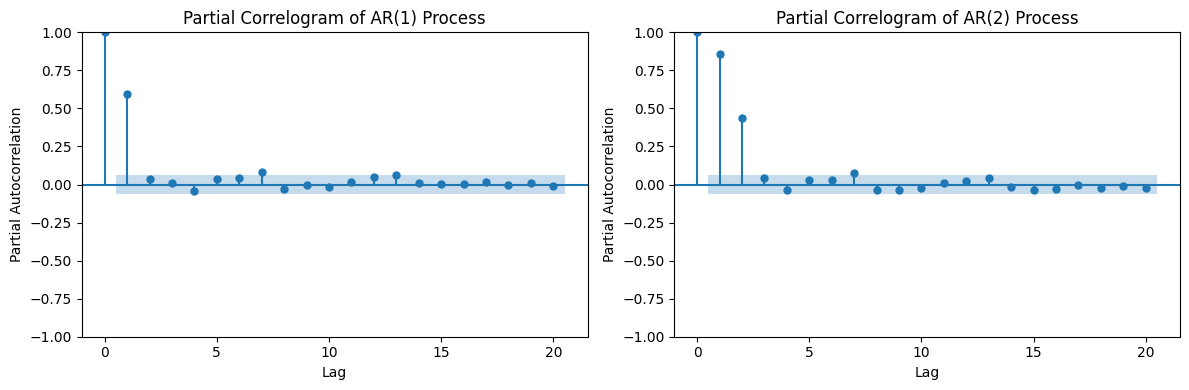
\includegraphics[width=250pt]{../img/09-ar-1-and-2.png}
        \caption{Figure 9.4:  Partial correlogram of an AR(1) and an AR(2) process.}
    \end{center}
\end{figure}


\subsection{Random walk}

An AR(1) process with \(\rho\) of \(1\) is called a \textbf{random walk\index{random walk}}:

\(x_t = x_{t-1} + \epsilon_t\)\\
\(x_t = x_{t-2} + \epsilon_{t-1} + \epsilon_t\)\\
\(x_t = x_0 + \sum_{i=0}^{t-1} \epsilon_{t-i}\)

Since the condition for stationary of variance is violated, it's non stationary time series.

\(Var(x_t) = Var(\sum_{i=0}^{t-1} \epsilon_{t-i}) = \sum_{i=0}^{t-1} Var(\epsilon_{t-i})\)\\
From \(\epsilon_i \sim i.i.d(0, \sigma^2)\), having \(t\) count of noise terms\\
\(Var(x_t) = t \sigma^2\) which is non constant but a function of time.

\subsection{SARIMAX}

SARIMAX is a commonly applied time series analysis technique, it is actually a combination of multiple techniques:

\begin{itemize}
    \item AR: Autoregression
    \item MA: Moving Average
    \item I: Adding differencing to ARMA
    \item S: Seasonality added it ARIMA
    \item X: External parameter added (moving from single variate to multi variate)
\end{itemize}

\section{Non linear modelling of time series data}

Linear models assume some form of linear relationship in time series. If the time series has some non linear relationship and is not purely a random walk or white noise we can try to fit a non linear model.

A number of machine learning techniques we discussed so far as well as new techniques developed for sequential data can be fit to model time series. If a model is successfully fit on a time series, it can be used for forecasting unseen/future values.

\subsection{Neural networks in time series}

One simple approach is to train a deep neural network with \(k\) inputs capturing the relationship among \(k\) consecutive samples in the time series. A challenge is that we might not know \(k\) but also that \(k\) might differ for a test dataset or even among training sets.

To support a variable number of inputs, which form a sequence, where previous values influence future or upcoming values, an extension of neural network has been developed called \textbf{recurrent neural network\index{recurrent neural network}} or \textbf{RNN\index{RNN}}. The difference between an RNN and a multilayer network is that these networks have \textbf{feedback loops\index{feedback loops}}.

Just as with multilayer network we define an input at position or time \(t\) as \(X_t\) which can be single value (scalar) or multiple values (vector). Assuming the more complex case, where we have multiple inputs at each moment \(t\), \(X_t\) would be a vector of dimension \(d_x\).

A common structure for RNN has a single hidden layer with a non linear activation function, noted with \(f_h\), also used for the feedback loop, and an output activation, noted with \(f_Y\). These two activation functions might be of different type, for example the hidden layer activation \(f_h\) might be a tanh function while the output activation \(f_Y\) might be a softmax function.

An RNN, similar to multilayer networks, has weights and biases. RNNs introduce one more set of weights, noted here with the matrix \(W_{hh}\) for the feedback loop, the output of a network would become an input as well. The hidden layer can have one or more neurons, we can note this number with \(d_h\). \(W_{hh}\), representing the weights between all neurons in the hidden layer to all other neurons, would be a square matrix with dimension \(d_h \times d_h\).

Similar to multi layer networks, we have weights associated with inputs which we can represent as a matrix \(W_{Xh}\) of dimension \(d_x \times d_h\), mapping inputs to hidden layer neurons. Using the activation for the hidden layer \(A_h\), the recurrent relationship can be written as:

\[h_t = A_h(W_{Xh} X_t + W_{hh} h_{t-1} + b_h)\]

Where \(b_h\) is the bias term for the hidden layer.The output of an RNN for time step \(t\) can be computed as:

\[Y_t = A_Y(W_{hY} h_t + b_Y)\]

The weight matrix \(W_{hY}\) that transforms the hidden state to the output space has the shape of \(d_h \times d_Y\), where \(d_Y\) is the dimensionality of the output. \(b_Y\) is the bias term for the output.

To combine the two formula into a single, more continuous formula, would be:
\[Y_t = A_Y(W_{hY} \times A_h(W_{xh} X_t + W_{hh} h_{t-1} + b_h) + b_o)\]


\begin{figure}[htbp]
    \begin{center}
        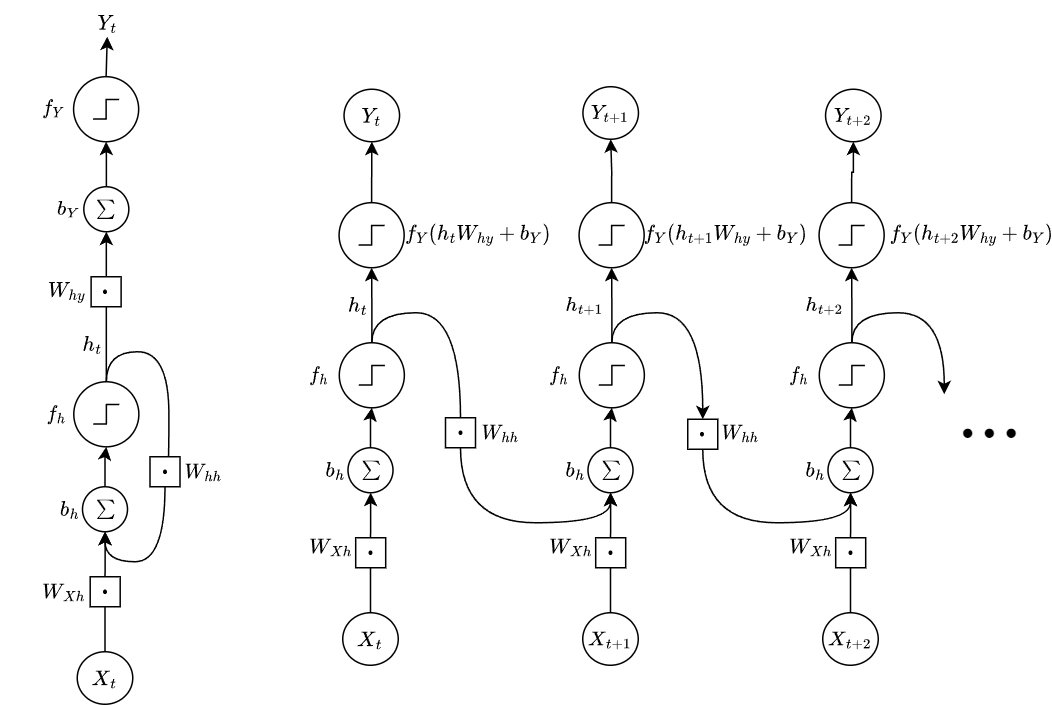
\includegraphics[width=300pt]{../img/09-rnn.png}
        \caption{Figure 9.5:  Left: structure of an RNN, right: unrolling of the network}
    \end{center}
\end{figure}


\textbf{Figure 9.5\index{Figure 9.5}} shows the RNN visually. On the left side we can see the feedback loop. This network can be unrolled by making copies of the network, in which case the feedback loop would become input for the next copy. This process is called unrolling and has been used by state of the art network at the time of writing this material. The right side of the diagram shows the unrolled version of the network.

\textbf{Modelling an AR(k) model with RNN\index{Modelling an AR(k) model with RNN}}

While it is not efficient to use RNN for an AR(k) process, it is a useful way to understand how RNN works and extends the AR process. Applying RNN would probably introduce unnecessary variance and overfit the model. But if we were to model an AR(k) process defined as \(x_t = \rho_0 + \rho_1 x_{t-1} + ... + \rho_k x_{t-k} + \epsilon\) the RNN would have the following properties:

\begin{itemize}
    \item Input would be a scalar, the value of the time series at time \(t-k\) leading up to \(t-1\). The output would also be a scalar, the prediction, or current value: \(x_t\).
    \item The hidden layer would need to have \(k\) activation functions, where both the hidden layer and output activation functions would be linear function: \(f_h(x) = f_Y(x) = x\) for all values of \(x\).
    \item The weights on the output layer would be the identity matrix \(I\), with each diagonal value of \(1\) and off diagonal element of \(0\)
    \item While multiple set of weights on the hidden layer could model an AR(k) process, a very straightforward option would be a diagonal matrix, where each diagonal element would be a coefficient of the AR(k) process: \(\rho_1 ... \rho_k\). The bias term would be equal to \(\rho_0\)
\end{itemize}

Such a recurrent network would be equivalent with the AR(k) process. If we were to train an actual RNN using samples from an AR(k), we would probably end up with a different but equivalent definition of weights, resulting from the random initialization of the network.

Notice the points that we simplified and if we are to utilize, can capture more complex relationships in the time series:

\begin{itemize}
    \item When we modelled an AR(k) process, we used only a small potion of the available weights. We can leverage off diagonal elements in the hidden layer as well as the weights in the output layer to create a more complex model.
    \item Non linear activation functions can capture non linear relationship between the points in time as well as in the output mapping. Interactions between the inputs can also be approximated
    \item Using identity matrix for weights as well as linear activation, we effectively removed the output layer.
    \item An RNN can handle multiple inputs and outputs.
\end{itemize}

\textbf{Considerations of RNN\index{Considerations of RNN}}

An RNN, even when we consider the unrolled version, still uses the same weights for each copy. To scale an RNN, the simplest way is to increase the neurons in the hidden layer. Another option is to stack multiple RNNs, the output of the first RNN would be the input of the second RNN and so forth.

RNNs provide a useful way to think about neural networks but in practice it's rarely used in it's simplest form. The biggest challenge of RNN is it's difficulty of training. In practice, the more we unroll an RNN network, will behave like a really deep neural network. All the difficulties of training deep neural networks arise in a magnified manners.

More specifically the issue is that weight training is unstable, leading to \textbf{vanishing\index{vanishing}} or \textbf{exploding gradients\index{exploding gradients}} problems. Considering a single weight in the hidden layer, noted with \(w\) and the input \(x\), a network unrolled \(n\) times, the loss function will contain the output of the network compared with the training data set, which in turn will have in it's formula the expression \(x w^n\). If \(n\) is large, e.g. 100, which can happen easily for time series inputs like price changes across time, the expression \(x w^n\) can become close to \(0\) if \(w < 1\) or very large for \(w > 1\). In the backpropagation process we calculate the gradient of the loss function, which will have similar behavior, resulting in the problem of vanishing gradient (\(n \gg 1, w < 1 \rightarrow w^n \approx 0\)) or exploding gradient (\(n \gg 1, w > 1 \rightarrow w^n \approx \infty\)).

To resolve the vanishing/exploding gradient issue, further variations of RNN has been proposed. Sepp Hochreiter and Jürgen Schmidhuber in their paper called "Long Short-Term Memory" defined \textbf{Long Short Term Memory\index{Long Short Term Memory}} networks, \textbf{LSTM\index{LSTM}} in brief. They applied gating mechanism and two tracks to maintain a long term memory and a short term memory, while keeping the network easier to train. In more recent years, the attention and transformer architecture has seen great results, outperforming LSTM in both ease of training and ability to maintain memory. Transformer architecture has seen great results being applied to time series, also allowing for multivariate time series forecasting, using other features available in the data. We will explore transformer architecture in the context of natural language processing and large language models, but the same architecture can be used for time series as well.

\subsection{Tree models in time series modelling}



\subsection{Trend and seasonality modelling - Facebook Prophet}


